\documentclass[11pt,a4paper]{article}

% --- Packages ---
\usepackage[margin=1in]{geometry}
\usepackage{tikz}
\usetikzlibrary{
  arrows.meta,
  positioning,
  shapes.geometric,
  shapes.multipart,
  fit,
  calc,
  backgrounds,
  chains,
  decorations.pathreplacing,
  automata,
  matrix
}
\usepackage{listings}
\usepackage{xcolor}
\usepackage{hyperref}
\usepackage{amsmath,amssymb}
\usepackage{booktabs}
\usepackage{enumitem}
\usepackage{fancyhdr}
\usepackage{titlesec}
\usepackage{tcolorbox}
\tcbuselibrary{listings,skins,breakable}
\usepackage{graphicx}
\usepackage{float}
\usepackage{caption}
\usepackage{tabularx}
\usepackage{multirow}

% --- Colors ---
\definecolor{cnblue}{HTML}{1A3A5C}
\definecolor{cnlight}{HTML}{4A90D9}
\definecolor{cngray}{HTML}{F5F5F5}
\definecolor{cngreen}{HTML}{2E7D32}
\definecolor{cnred}{HTML}{C62828}
\definecolor{cnorange}{HTML}{E65100}
\definecolor{cnpurple}{HTML}{6A1B9A}
\definecolor{cnteal}{HTML}{00695C}

% --- Code listing style ---
\lstdefinestyle{typescript}{
  language=Java,
  basicstyle=\ttfamily\footnotesize,
  keywordstyle=\color{cnblue}\bfseries,
  stringstyle=\color{cngreen},
  commentstyle=\color{gray}\itshape,
  breaklines=true,
  frame=none,
  showstringspaces=false,
  tabsize=2,
  morekeywords={async,await,const,let,interface,type,export,import,from,extends,
    implements,readonly,string,number,boolean,void,Promise,Map,undefined,
    Record,Uint8Array,Date,Array}
}

\lstdefinestyle{protobuf}{
  basicstyle=\ttfamily\footnotesize,
  keywordstyle=\color{cnblue}\bfseries,
  stringstyle=\color{cngreen},
  commentstyle=\color{gray}\itshape,
  breaklines=true,
  frame=none,
  showstringspaces=false,
  morekeywords={message,optional,repeated,string,uint32,uint64,bytes,enum,map,
    import,syntax,package,oneof}
}

% --- Code box environment ---
\newtcblisting{codebox}[2][]{
  colback=cngray,
  colframe=cnblue!60,
  listing only,
  listing options={style=#2,#1},
  left=6pt,
  right=6pt,
  top=4pt,
  bottom=4pt,
  boxrule=0.5pt,
  breakable
}

% --- Definition box ---
\newtcolorbox{defbox}[1]{
  colback=cnblue!5,
  colframe=cnblue!60,
  fonttitle=\bfseries,
  title=#1,
  boxrule=0.5pt
}

% --- Warning box ---
\newtcolorbox{warnbox}[1]{
  colback=cnorange!5,
  colframe=cnorange!60,
  fonttitle=\bfseries,
  title=#1,
  boxrule=0.5pt
}

% --- Research box ---
\newtcolorbox{researchbox}[1]{
  colback=cnpurple!5,
  colframe=cnpurple!60,
  fonttitle=\bfseries,
  title=#1,
  boxrule=0.5pt
}

% --- Header/Footer ---
\pagestyle{fancy}
\fancyhf{}
\fancyhead[L]{\small\textcolor{cnblue}{DED Multi-Party State Protocol}}
\fancyhead[R]{\small\textcolor{cnblue}{Technical Proposal v0.1}}
\fancyfoot[C]{\thepage}
\renewcommand{\headrulewidth}{0.4pt}

% --- Title formatting ---
\titleformat{\section}{\Large\bfseries\color{cnblue}}{\thesection}{1em}{}
\titleformat{\subsection}{\large\bfseries\color{cnblue!80}}{\thesubsection}{1em}{}
\titleformat{\subsubsection}{\normalsize\bfseries\color{cnblue!60}}{\thesubsubsection}{1em}{}

% --- Document ---
\begin{document}

% ============================================================================
% TITLE PAGE
% ============================================================================
\begin{titlepage}
\centering
\vspace*{1.5cm}

{\Huge\bfseries\color{cnblue} DED Multi-Party\\ State Protocol\par}
\vspace{0.5cm}
{\Large\color{cnblue!70} Verifiable Multi-Party Computation\\ via Committed State Tries\par}
\vspace{0.8cm}
{\large Technical Proposal --- v0.1\par}
\vspace{0.3cm}
{\large February 2026\par}

\vspace{1.5cm}

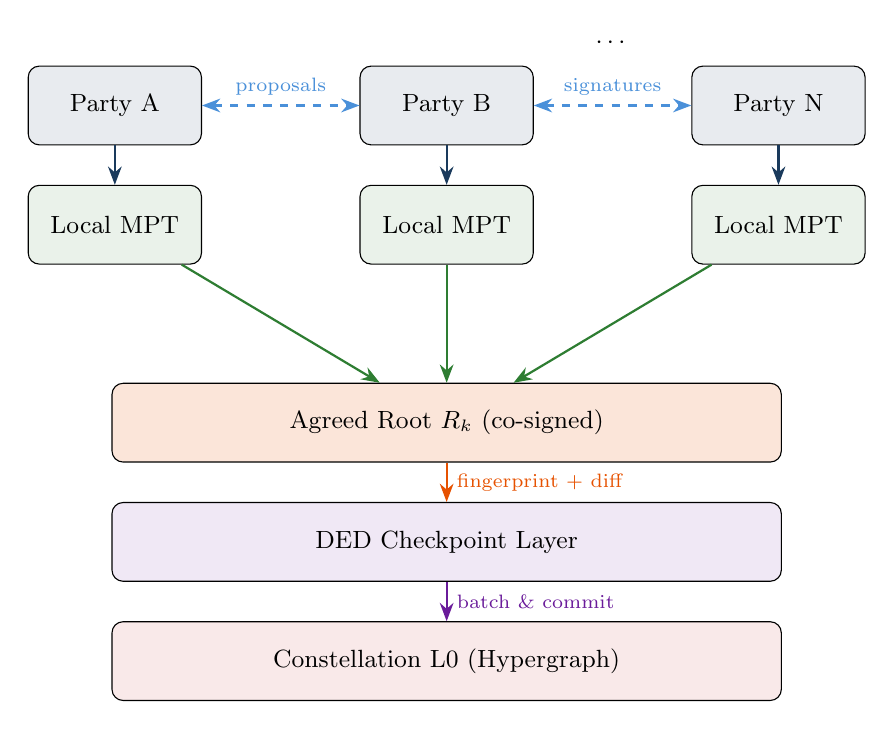
\begin{tikzpicture}[
  node distance=0.5cm and 1.2cm,
  every node/.style={font=\small}
]
  % Parties
  \node[draw, rounded corners, fill=cnblue!10, minimum width=2.2cm, minimum height=1cm]
    (partyA) {Party A};
  \node[draw, rounded corners, fill=cnblue!10, minimum width=2.2cm, minimum height=1cm,
    right=2cm of partyA] (partyB) {Party B};
  \node[draw, rounded corners, fill=cnblue!10, minimum width=2.2cm, minimum height=1cm,
    right=2cm of partyB] (partyN) {Party N};

  % Local tries
  \node[draw, rounded corners, fill=cngreen!10, minimum width=2.2cm, minimum height=1cm,
    below=of partyA] (trieA) {Local MPT};
  \node[draw, rounded corners, fill=cngreen!10, minimum width=2.2cm, minimum height=1cm,
    below=of partyB] (trieB) {Local MPT};
  \node[draw, rounded corners, fill=cngreen!10, minimum width=2.2cm, minimum height=1cm,
    below=of partyN] (trieN) {Local MPT};

  % Agreed root
  \node[draw, rounded corners, fill=cnorange!15, minimum width=8.5cm, minimum height=1cm,
    below=1.5cm of trieB] (agreed) {Agreed Root $R_k$ (co-signed)};

  % DED
  \node[draw, rounded corners, fill=cnpurple!10, minimum width=8.5cm, minimum height=1cm,
    below=of agreed] (ded) {DED Checkpoint Layer};

  % Chain
  \node[draw, rounded corners, fill=cnred!10, minimum width=8.5cm, minimum height=1cm,
    below=of ded] (chain) {Constellation L0 (Hypergraph)};

  % Arrows
  \draw[-{Stealth}, thick, cnblue] (partyA) -- (trieA);
  \draw[-{Stealth}, thick, cnblue] (partyB) -- (trieB);
  \draw[-{Stealth}, thick, cnblue] (partyN) -- (trieN);

  \draw[-{Stealth}, thick, cngreen] (trieA) -- (agreed);
  \draw[-{Stealth}, thick, cngreen] (trieB) -- (agreed);
  \draw[-{Stealth}, thick, cngreen] (trieN) -- (agreed);

  \draw[-{Stealth}, thick, cnorange] (agreed) -- node[right, font=\scriptsize] {fingerprint + diff} (ded);
  \draw[-{Stealth}, thick, cnpurple] (ded) -- node[right, font=\scriptsize] {batch \& commit} (chain);

  % P2P arrows
  \draw[{Stealth}-{Stealth}, dashed, cnlight, thick] (partyA) -- node[above, font=\scriptsize]
    {proposals} (partyB);
  \draw[{Stealth}-{Stealth}, dashed, cnlight, thick] (partyB) -- node[above, font=\scriptsize]
    {signatures} (partyN);

  % Dots between B and N at the party level
  \node at ($(partyB)!0.5!(partyN)$) [yshift=0.8cm] {$\cdots$};

\end{tikzpicture}

\vspace{1.5cm}

\begin{tabular}{ll}
\textbf{Status:} & Draft \\
\textbf{Authors:} & Constellation Network Engineering \\
\textbf{Extends:} & DED Agent WorldState v0.1 \\
\textbf{Package:} & \texttt{@constellation-network/ded-agent-worldstate} \\
\textbf{Dependencies:} & \texttt{@constellation-network/ded-sdk}, \texttt{@constellation-network/metagraph-sdk} \\
\end{tabular}

\end{titlepage}

\tableofcontents
\newpage

% ============================================================================
\section{Executive Summary}
% ============================================================================

This proposal extends the DED Agent WorldState (v1) from single-party state
commitment to a \textbf{Multi-Party Verifiable State Protocol (MPVSP)} where
$N$ parties maintain a shared Merkle Patricia Trie, agree on state transitions
via co-signature, and checkpoint committed roots to the DED notarization
platform.

The core insight is that DED serves as a \textbf{periodic checkpoint layer}
--- not a real-time consensus engine. Parties advance state off-chain at
communication speed (sub-second), while DED provides the cryptographic anchoring
that makes historical state provable and disputes resolvable. This two-layer
architecture mirrors the relationship between Layer~2 rollups and Layer~1
settlement, but without requiring smart contracts or on-chain execution.

\textbf{Key design decisions:}
\begin{itemize}[nosep]
  \item \textbf{Zero server changes}: The entire protocol lives in the client
    SDK. DED's existing fingerprint and upload APIs are used unmodified.
  \item \textbf{Transport-agnostic}: The SDK defines a \texttt{Transport}
    interface; parties bring their own communication channel (WebSocket, HTTP,
    MQTT, etc.).
  \item \textbf{Git-referenced transition functions}: Allowed state transitions
    are defined by code in a versioned repository. The protocol spec references
    a git commit hash; the SDK loads and executes validators from that code.
  \item \textbf{State diffs via \texttt{/upload}}: Each committed transition
    includes the state diff uploaded as a document, enabling any party to
    reconstruct state from the DED-committed history.
  \item \textbf{Phased delivery}: Phase~1 targets bilateral (N=2) protocols.
    Phase~2 extends to small consortia (N=3--10). Phase~3 introduces
    zero-knowledge property proofs and WASM transition functions.
\end{itemize}


% ============================================================================
\section{Motivation}
% ============================================================================

The v1 WorldState proposal established that a single autonomous agent can
maintain a verifiable internal state by committing MPT roots to DED. This
solved the \emph{self-verification} problem: an agent proving the integrity of
its own state history.

However, real-world workflows rarely involve a single party acting alone.
Supply chain handoffs require shipper and receiver agreement. Escrow
transactions need buyer, seller, and arbiter coordination. Regulatory
compliance demands multi-party attestation. In each case, the critical question
extends from ``what did \emph{I} know?'' to ``what did \emph{we} agree?''

\subsection{The Multi-Party Trust Gap}

When multiple parties must agree on shared state, three new challenges emerge
beyond single-party commitment:

\begin{enumerate}[leftmargin=2cm]
  \item \textbf{Agreement} --- How do parties reach consensus on state
    transitions without a central authority? Who proposes changes, and how are
    conflicts resolved?
  \item \textbf{Accountability} --- If a party violates the agreed protocol,
    how is this detected and proven to third parties? Can we produce
    cryptographic evidence of misbehavior?
  \item \textbf{Verifiability} --- Can an external auditor verify the
    multi-party interaction history without trusting any individual party? Can
    parties prove properties about their state without revealing the state
    itself?
\end{enumerate}

\subsection{Why DED as the Foundation}

DED provides three properties that make it uniquely suited as the anchoring
layer for multi-party protocols:

\begin{itemize}
  \item \textbf{Neutral commitment log}: DED is operated by a network
    (Constellation Hypergraph), not a single party. Commitments are
    tamper-evident and publicly verifiable.
  \item \textbf{Document storage}: The \texttt{POST /v1/fingerprints/upload}
    route provides hash-verified document storage alongside fingerprint
    commitments, enabling state diff persistence.
  \item \textbf{Existing proof infrastructure}: DED already generates MPT
    inclusion proofs (\texttt{GET /v1/fingerprints/\{hash\}/proof}),
    providing the cryptographic foundation for dispute resolution.
\end{itemize}


% ============================================================================
\section{Relationship to v1}
% ============================================================================

This proposal is a strict extension of the v1 Agent WorldState. All v1
concepts --- per-stream MPTs, chain linking via \texttt{documentId}, checkpoint
and recovery --- remain unchanged. Multi-party state is built \emph{on top of}
single-party streams:

\begin{defbox}{Architectural Principle}
A multi-party protocol instance is an orchestration of single-party streams.
Each party writes to their own stream. Shared state is written by the leader
after quorum is reached. The protocol layer coordinates which streams are
written and when.
\end{defbox}

\noindent Concretely, a protocol instance with members \texttt{[A, B, C]} maps to
the following v1 streams:

\begin{center}
\begin{tabular}{lll}
\toprule
\textbf{Logical Path} & \textbf{v1 Stream} & \textbf{Writer} \\
\midrule
\texttt{/protocol/*} & \texttt{stream(proto, ``protocol'', specHash)} & Genesis only \\
\texttt{/state/A/*} & \texttt{stream(proto, ``A'', specHash)} & Party A \\
\texttt{/state/B/*} & \texttt{stream(proto, ``B'', specHash)} & Party B \\
\texttt{/state/C/*} & \texttt{stream(proto, ``C'', specHash)} & Party C \\
\texttt{/shared/*} & \texttt{stream(proto, ``shared'', specHash)} & Leader (after quorum) \\
\texttt{/audit/*} & \texttt{stream(proto, ``audit'', specHash)} & Leader (after quorum) \\
\bottomrule
\end{tabular}
\end{center}

\noindent The protocol-level MPT is a \textbf{unified trie} that spans all
these logical paths. Each party maintains a complete local copy of this
unified trie. The v1 per-stream MPTs provide the DED-committed chain for each
logical partition; the protocol-level MPT is the single root that binds them
all.


% ============================================================================
\section{System Architecture}
% ============================================================================

\subsection{Two-Layer State Model}

The protocol operates across two distinct state layers with different
consistency and finality guarantees:

\begin{figure}[H]
\centering
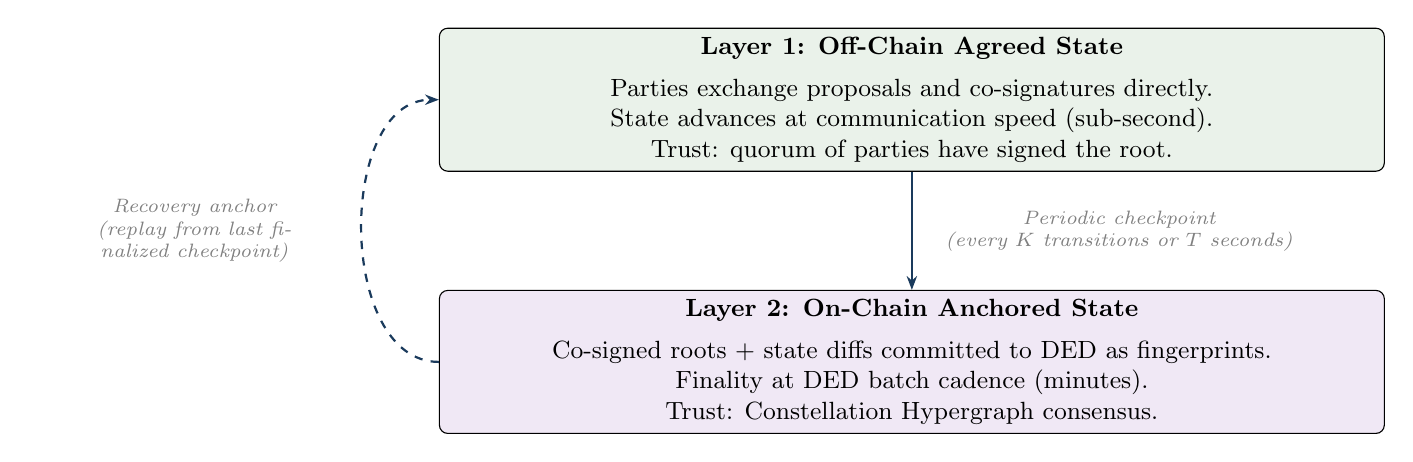
\begin{tikzpicture}[
  node distance=1.2cm,
  layer/.style={draw, rounded corners=3pt, minimum width=12cm, minimum height=1.8cm,
    font=\small, align=center},
  arrow/.style={-{Stealth[length=5pt]}, thick},
  note/.style={font=\scriptsize\itshape, text=gray}
]

  \node[layer, fill=cngreen!10] (l1) {
    \textbf{Layer 1: Off-Chain Agreed State} \\[4pt]
    Parties exchange proposals and co-signatures directly. \\
    State advances at communication speed (sub-second). \\
    Trust: quorum of parties have signed the root.
  };

  \node[layer, fill=cnpurple!10, below=1.5cm of l1] (l2) {
    \textbf{Layer 2: On-Chain Anchored State} \\[4pt]
    Co-signed roots + state diffs committed to DED as fingerprints. \\
    Finality at DED batch cadence (minutes). \\
    Trust: Constellation Hypergraph consensus.
  };

  \draw[arrow, cnblue] (l1) -- node[right, note, text width=5cm, align=center]
    {Periodic checkpoint\\(every $K$ transitions or $T$ seconds)} (l2);

  \draw[arrow, cnblue, dashed] (l2.west) to[out=180, in=180]
    node[left, note, text width=4cm, align=center]
    {Recovery anchor\\(replay from last finalized checkpoint)} (l1.west);

\end{tikzpicture}
\caption{Two-layer state model. Layer~1 is fast but requires party
availability. Layer~2 is slow but provides durable, publicly verifiable
anchoring.}
\label{fig:twolayer}
\end{figure}

\begin{warnbox}{The Finality Gap}
Between off-chain agreement and DED confirmation, there is a window of 1--5
minutes where the agreed state is not yet anchored. During this window,
equivocation is theoretically possible. The protocol mitigates this via
\textbf{epoch numbering} and \textbf{previousRoot chaining}
(Section~\ref{sec:security}).
\end{warnbox}

\subsection{Architecture Diagram}

\begin{figure}[H]
\centering
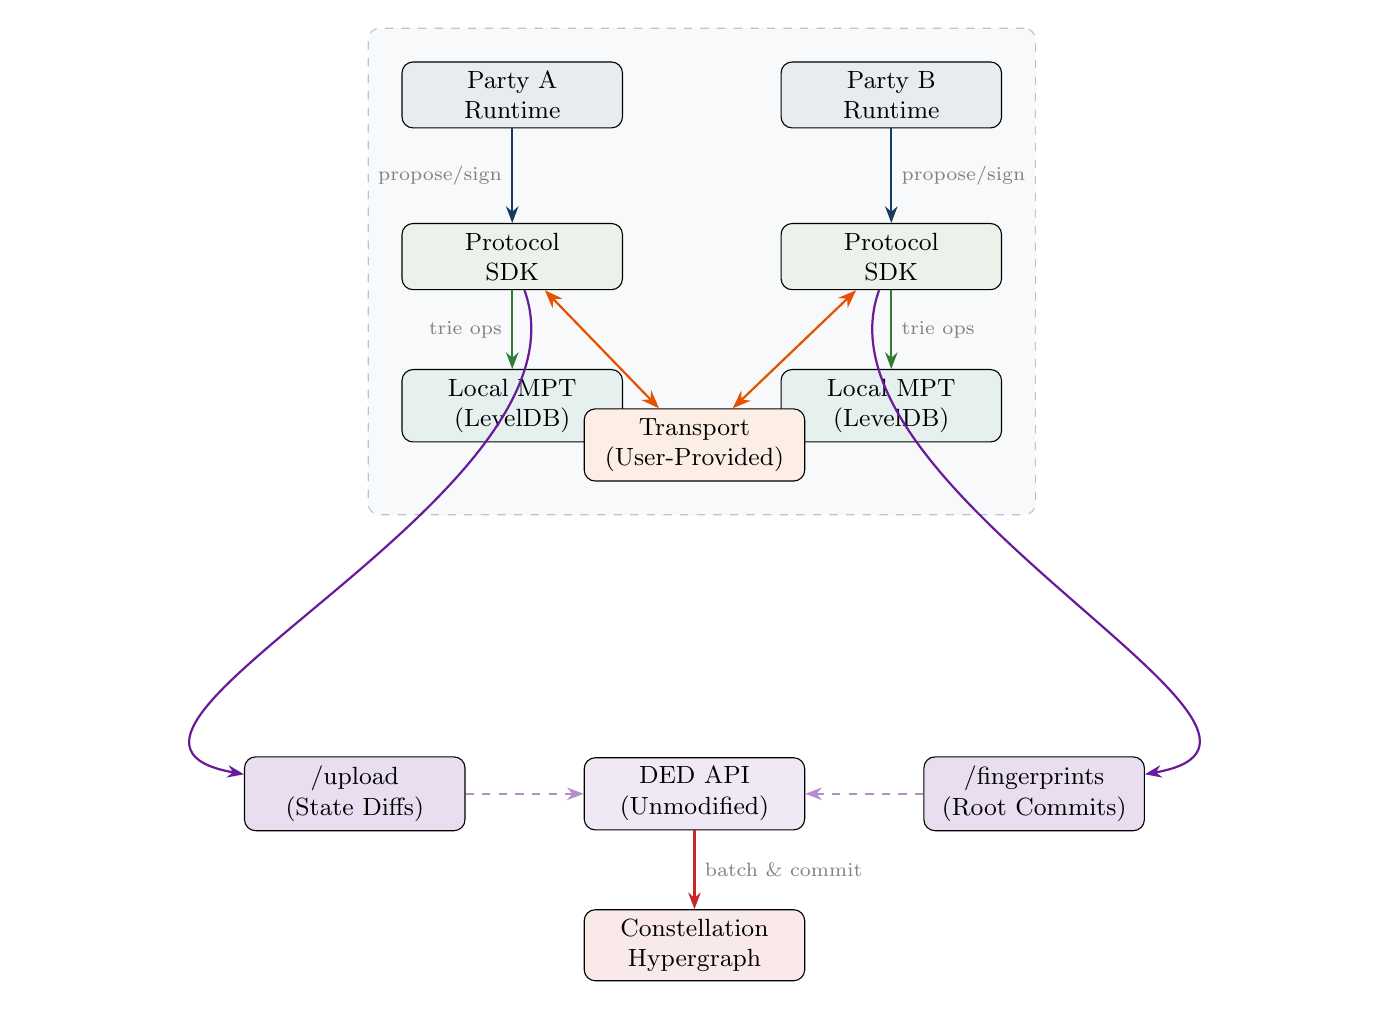
\begin{tikzpicture}[
  node distance=1cm and 1.8cm,
  box/.style={draw, rounded corners=4pt, minimum width=2.8cm, minimum height=0.8cm,
    font=\small, align=center},
  arrow/.style={-{Stealth[length=6pt]}, thick},
  label/.style={font=\scriptsize, text=gray}
]

  % --- Party Layer ---
  \node[box, fill=cnblue!10] (pA) {Party A\\Runtime};
  \node[box, fill=cnblue!10, right=2cm of pA] (pB) {Party B\\Runtime};

  % --- SDK Layer ---
  \node[box, fill=cngreen!10, below=1.2cm of pA] (sdkA) {Protocol\\SDK};
  \node[box, fill=cngreen!10, below=1.2cm of pB] (sdkB) {Protocol\\SDK};

  % --- Local State ---
  \node[box, fill=cnteal!10, below=of sdkA] (mptA) {Local MPT\\(LevelDB)};
  \node[box, fill=cnteal!10, below=of sdkB] (mptB) {Local MPT\\(LevelDB)};

  % --- Transport ---
  \node[box, fill=cnorange!10, below right=1.5cm and -0.5cm of sdkA] (transport)
    {Transport\\(User-Provided)};

  % --- DED ---
  \node[box, fill=cnpurple!10, below=3.5cm of transport] (ded) {DED API\\(Unmodified)};
  \node[box, fill=cnpurple!15, left=1.5cm of ded] (upload) {/upload\\(State Diffs)};
  \node[box, fill=cnpurple!15, right=1.5cm of ded] (fp) {/fingerprints\\(Root Commits)};

  % --- Chain ---
  \node[box, fill=cnred!10, below=of ded] (chain) {Constellation\\Hypergraph};

  % Party -> SDK
  \draw[arrow, cnblue] (pA) -- node[left, label] {propose/sign} (sdkA);
  \draw[arrow, cnblue] (pB) -- node[right, label] {propose/sign} (sdkB);

  % SDK -> MPT
  \draw[arrow, cngreen] (sdkA) -- node[left, label] {trie ops} (mptA);
  \draw[arrow, cngreen] (sdkB) -- node[right, label] {trie ops} (mptB);

  % SDK <-> Transport
  \draw[{Stealth}-{Stealth}, thick, cnorange] (sdkA) -- (transport);
  \draw[{Stealth}-{Stealth}, thick, cnorange] (sdkB) -- (transport);

  % SDK -> DED
  \draw[arrow, cnpurple] (sdkA) to[out=-70, in=170] (upload);
  \draw[arrow, cnpurple] (sdkB) to[out=-110, in=10] (fp);

  % DED internal
  \draw[arrow, cnpurple!50, dashed] (upload) -- (ded);
  \draw[arrow, cnpurple!50, dashed] (fp) -- (ded);

  % DED -> Chain
  \draw[arrow, cnred] (ded) -- node[right, label] {batch \& commit} (chain);

  % Background boxes
  \begin{scope}[on background layer]
    \node[draw=cnblue!30, dashed, rounded corners, fill=cnblue!3,
      fit=(pA)(pB)(sdkA)(sdkB)(mptA)(mptB)(transport),
      inner sep=12pt, label={[font=\footnotesize\bfseries,
      text=cnblue]above:Client SDK (Zero Server Changes)}] {};
  \end{scope}

\end{tikzpicture}
\caption{Multi-party architecture. The entire protocol runs client-side. DED
serves as an unmodified checkpoint and storage layer.}
\label{fig:arch}
\end{figure}


% ============================================================================
\section{Protocol Specification}
% ============================================================================

\subsection{Protocol Spec}

A \texttt{ProtocolSpec} defines the rules, participants, and allowed
transitions for a multi-party interaction. The spec is a structured object
whose SHA-256 hash serves as its identity:

\begin{codebox}{typescript}
interface ProtocolSpec {
  name: string;                          // Human-readable name
  version: number;                       // Spec version (monotonic)
  codeRef: {
    type: 'git';
    repository: string;                  // Git repository URL
    commit: string;                      // Full SHA-1 commit hash
    entrypoint: string;                  // Path to transition module
  };
  members: Record<string, MemberSpec>;   // memberId -> spec
  transitions: Record<string, TransitionSchema>;
  quorum: QuorumRule;
  config: ProtocolConfig;
}

interface MemberSpec {
  publicKey: string;                     // SECP256K1 public key (hex)
  roles: string[];                       // Authorized transition types
}

interface TransitionSchema {
  proposer: string | string[];           // Who may propose
  requiredSigners: string[] | QuorumRule; // Who must co-sign
  statePaths: {
    reads: string[];                     // Paths read during validation
    writes: string[];                    // Paths written on commit
  };
}

type QuorumRule =
  | { type: 'all' }                      // All members
  | { type: 'threshold'; min: number }   // At least min members
  | { type: 'roles'; require: string[] } // Specific members by ID

interface ProtocolConfig {
  checkpointInterval: number;            // Transitions between DED commits
  proposalTimeoutMs: number;             // ms before proposal expires
  leaderElection: 'round-robin' | 'proposer-defined';
  disputeWindowMs: number;               // ms for dispute submission
}
\end{codebox}

\begin{defbox}{Spec Hash}
$\text{specHash} = \text{SHA-256}(\text{RFC8785}(\text{ProtocolSpec}))$

\medskip\noindent
The spec hash is computed over the canonical JSON serialization of the
\texttt{ProtocolSpec} object. All parties must compute the same hash to
participate. The spec hash appears as the \texttt{appId} in DED fingerprint
submissions, binding each commitment to its governing protocol.
\end{defbox}

\subsection{Schema-Defined State Paths}
\label{sec:paths}

The protocol's unified MPT uses a hierarchical path namespace with reserved
prefixes:

\begin{figure}[H]
\centering
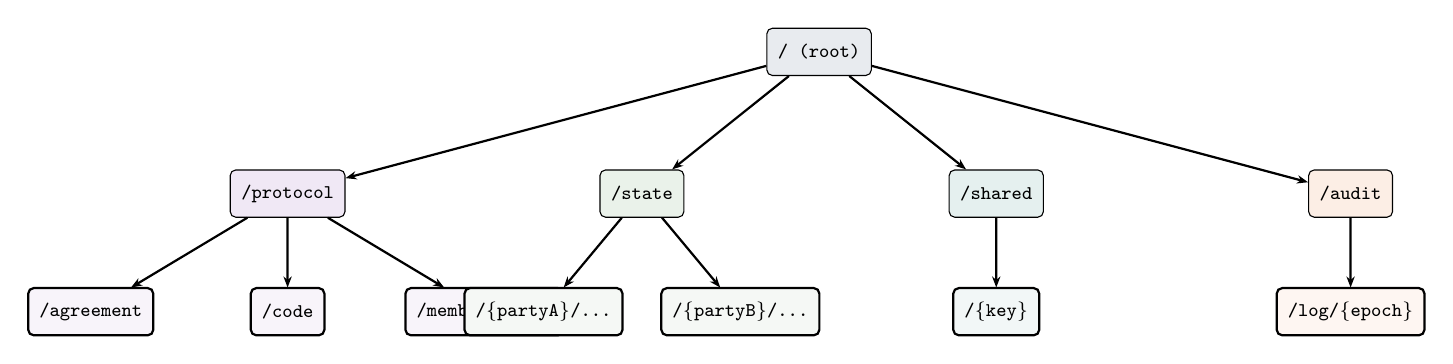
\begin{tikzpicture}[
  level 1/.style={sibling distance=4.5cm, level distance=1.8cm},
  level 2/.style={sibling distance=2.5cm, level distance=1.5cm},
  level 3/.style={sibling distance=2cm, level distance=1.5cm},
  every node/.style={draw, rounded corners=2pt, font=\ttfamily\scriptsize,
    minimum height=0.6cm, inner sep=4pt},
  edge from parent/.style={draw, -{Stealth[length=4pt]}, thick}
]

  \node[fill=cnblue!10] {/ (root)}
    child { node[fill=cnpurple!10] {/protocol}
      child { node[fill=cnpurple!5] {/agreement} }
      child { node[fill=cnpurple!5] {/code} }
      child { node[fill=cnpurple!5] {/members/\{id\}} }
    }
    child { node[fill=cngreen!10] {/state}
      child { node[fill=cngreen!5] {/\{partyA\}/...} }
      child { node[fill=cngreen!5] {/\{partyB\}/...} }
    }
    child { node[fill=cnteal!10] {/shared}
      child { node[fill=cnteal!5] {/\{key\}} }
    }
    child { node[fill=cnorange!10] {/audit}
      child { node[fill=cnorange!5] {/log/\{epoch\}} }
    };

\end{tikzpicture}
\caption{Hierarchical path namespace in the unified protocol MPT.}
\label{fig:paths}
\end{figure}

\begin{table}[H]
\centering
\begin{tabularx}{\textwidth}{lllX}
\toprule
\textbf{Prefix} & \textbf{Writer} & \textbf{Mutability} & \textbf{Contents} \\
\midrule
\texttt{/protocol/agreement} & Genesis & Immutable & Hash of legal/commercial terms \\
\texttt{/protocol/code} & Genesis & Immutable\textsuperscript{*} & Git reference (repo + commit) \\
\texttt{/protocol/members/\{id\}} & Genesis\textsuperscript{*} & Append-only & Public key, roles, status \\
\texttt{/protocol/config} & Genesis & Immutable\textsuperscript{*} & Quorum rules, timeouts, etc. \\
\texttt{/state/\{partyId\}/...} & Party owner & Mutable & Party-local application state \\
\texttt{/shared/...} & Leader & Mutable & Jointly-owned state (requires quorum) \\
\texttt{/audit/log/\{epoch\}} & Leader & Append-only & Transition receipts \\
\bottomrule
\end{tabularx}
\caption{Path namespace registry. \textsuperscript{*}Mutable only via
protocol upgrade transitions (Section~\ref{sec:upgrades}).}
\label{tab:paths}
\end{table}

\subsubsection{Path Encoding}

Logical paths are mapped to the 128-hex-char MPT key format required by the
DED evidence path structure. The mapping uses deterministic UUID~v5 derivation
from path components:

\[
  \text{mptKey} = \text{hex}\Big(
    \text{UUID5}(\text{instanceId})_{16\text{B}} \|
    \text{UUID5}(\text{pathSegment}_1)_{16\text{B}} \|
    \text{UUID5}(\text{pathSegment}_2)_{16\text{B}} \|
    \text{UUID5}(\text{pathSegment}_3)_{16\text{B}}
  \Big)
\]

This preserves compatibility with the server-side \texttt{PathEvidenceCalculator}
format (\texttt{tenantId + streamId + appId + eventId}) while supporting
arbitrary logical hierarchies.

\subsection{Transition Functions}
\label{sec:transitions}

Transition functions define the allowed state mutations. They are referenced
by a git commit hash in the \texttt{ProtocolSpec} and loaded as JavaScript/TypeScript
modules by the SDK at runtime.

\begin{codebox}{typescript}
// Transition module (referenced by ProtocolSpec.codeRef)
// Repository: github.com/acme/supply-chain-protocol
// Entrypoint: src/transitions/index.ts

import { z } from 'zod';
import type { TransitionModule, StateReader } from
  '@constellation-network/ded-agent-worldstate/protocol';

export const shipment_dispatched: TransitionModule = {
  schema: z.object({
    trackingId: z.string().min(1),
    dispatchedAt: z.string().datetime(),
    items: z.array(z.object({
      sku: z.string(),
      quantity: z.number().int().positive(),
    })),
  }),

  validate: async (state: StateReader, data: unknown) => {
    const parsed = shipment_dispatched.schema.parse(data);
    const existing = await state.read(
      `/state/shipper/dispatches/${parsed.trackingId}`
    );
    if (existing !== null) {
      return { valid: false, error: 'Duplicate dispatch' };
    }
    return { valid: true };
  },

  apply: async (state: StateWriter, data: unknown) => {
    const parsed = shipment_dispatched.schema.parse(data);
    await state.write(
      `/state/shipper/dispatches/${parsed.trackingId}`,
      { ...parsed, status: 'dispatched' }
    );
  },
};
\end{codebox}

\begin{defbox}{Determinism Requirement}
Transition functions \textbf{must be pure and deterministic}. Given the same
pre-state and input, every party must compute the same post-state. The SDK
enforces this by:
\begin{itemize}[nosep]
  \item Providing a sandboxed \texttt{StateReader}/\texttt{StateWriter} that
    intercepts all state access.
  \item Prohibiting side effects (no network, no filesystem, no randomness).
  \item Recording all read paths as witnesses for dispute resolution.
\end{itemize}
\end{defbox}

\begin{researchbox}{Future Direction: WASM Transition Functions}
JavaScript transition functions are convenient but have known determinism
risks across runtimes (floating-point handling, string collation, etc.). A
future version may support WebAssembly (WASM) modules as transition functions,
providing:
\begin{itemize}[nosep]
  \item Cross-platform deterministic execution
  \item Language-agnostic (Rust, Go, C compiled to WASM)
  \item Sandboxed by design (no host access without explicit imports)
  \item Formally verifiable execution semantics
\end{itemize}
The \texttt{ProtocolSpec.codeRef} would gain a \texttt{type: 'wasm'} variant
pointing to a WASM binary with a known hash.
\end{researchbox}


\subsection{Protocol Genesis}
\label{sec:genesis}

A protocol instance is created through a multi-step genesis ceremony:

\begin{enumerate}[nosep]
  \item \textbf{Spec Agreement}: All parties obtain the same
    \texttt{ProtocolSpec} (e.g., via a shared repository or direct exchange)
    and verify its hash matches.
  \item \textbf{Genesis Proposal}: The initiating party constructs the genesis
    MPT containing:
    \begin{itemize}[nosep]
      \item \texttt{/protocol/agreement} $\gets$ \texttt{H(terms\_document)}
      \item \texttt{/protocol/code} $\gets$ \texttt{codeRef} from spec
      \item \texttt{/protocol/members/\{id\}} $\gets$ member specs
      \item \texttt{/protocol/config} $\gets$ protocol configuration
    \end{itemize}
  \item \textbf{Co-Signature}: All members sign the genesis root. This is the
    only transition that \emph{always} requires unanimity, regardless of the
    configured quorum.
  \item \textbf{DED Commitment}: The genesis root is submitted to DED as the
    first fingerprint in the protocol's chain, with:
    \begin{itemize}[nosep]
      \item \texttt{documentId} = \texttt{mpvsp:\{instanceId\}:epoch:0}
      \item \texttt{documentRef} = genesis MPT root hash
      \item \texttt{proofs} = all members' signatures
    \end{itemize}
  \item \textbf{State Diff Upload}: The full genesis state is uploaded via
    \texttt{POST /v1/fingerprints/upload} as the initial state snapshot.
\end{enumerate}

\subsection{State Evolution}
\label{sec:evolution}

After genesis, state evolves through a propose--validate--sign--commit cycle:

\begin{figure}[H]
\centering
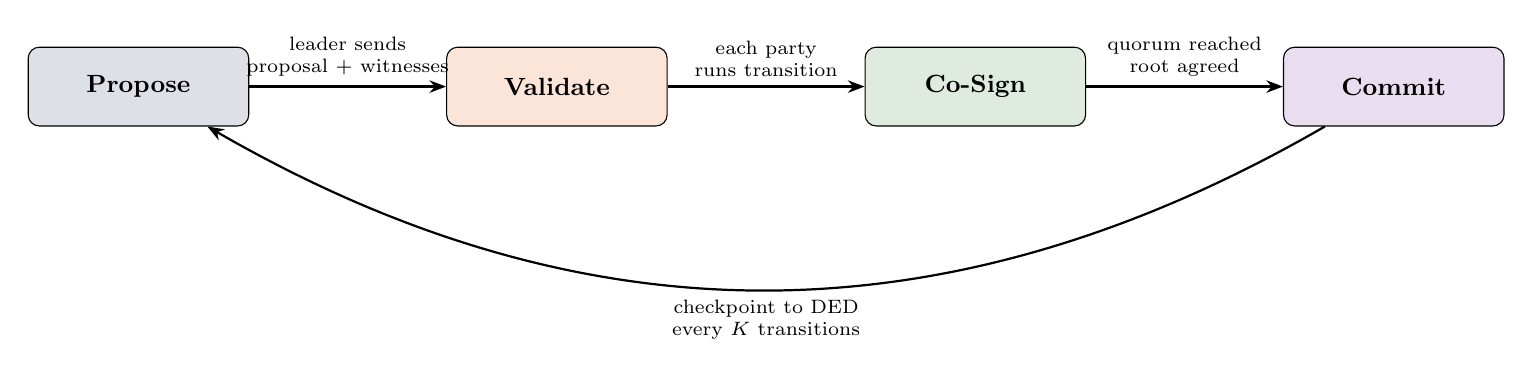
\begin{tikzpicture}[
  node distance=2.5cm,
  state/.style={draw, rounded corners=4pt, minimum width=2.8cm, minimum height=1cm,
    font=\small\bfseries, align=center},
  every edge/.style={draw, thick, -{Stealth[length=6pt]}},
  label/.style={font=\scriptsize, align=center}
]

  \node[state, fill=cnblue!15] (propose) {Propose};
  \node[state, fill=cnorange!15, right=of propose] (validate) {Validate};
  \node[state, fill=cngreen!15, right=of validate] (sign) {Co-Sign};
  \node[state, fill=cnpurple!15, right=of sign] (commit) {Commit};

  \draw (propose) edge[above] node[label] {leader sends\\proposal + witnesses} (validate);
  \draw (validate) edge[above] node[label] {each party\\runs transition} (sign);
  \draw (sign) edge[above] node[label] {quorum reached\\root agreed} (commit);

  % Loop back
  \draw (commit) edge[bend left=30, below] node[label, text width=3cm]
    {checkpoint to DED\\every $K$ transitions} (propose);

\end{tikzpicture}
\caption{State transition lifecycle. The cycle repeats for each epoch.}
\label{fig:lifecycle}
\end{figure}

\textbf{Detailed lifecycle for epoch $k$:}

\begin{enumerate}[nosep]
  \item \textbf{Leader Selection}: For epoch $k$, the leader is
    $\text{members}[k \bmod N]$ (round-robin by sorted member ID). If the
    designated leader does not propose within \texttt{proposalTimeoutMs}, the
    next member becomes leader.

  \item \textbf{Propose}: The leader constructs a \texttt{Proposal}:
    \begin{itemize}[nosep]
      \item Transition name and input data (validated against schema)
      \item Pre-state root $R_{k-1}$ (the current agreed root)
      \item Post-state root $R_k$ (computed by applying the transition)
      \item Epoch number $k$ (monotonically increasing)
      \item State witnesses: MPT inclusion proofs for all paths read during
        validation, and the key-value diffs for all paths written
      \item Leader's signature over $(R_{k-1}, R_k, k, \text{transitionHash})$
    \end{itemize}

  \item \textbf{Validate}: Each party independently:
    \begin{itemize}[nosep]
      \item Verifies $R_{k-1}$ matches their local root
      \item Verifies the state witnesses against $R_{k-1}$
      \item Loads the transition function from the code reference
      \item Executes the transition with the witnessed pre-state and input
      \item Computes $R_k'$ from the resulting state changes
      \item Verifies $R_k' = R_k$ (the proposed root matches their computation)
    \end{itemize}

  \item \textbf{Co-Sign}: If validation passes, the party signs
    $(R_{k-1}, R_k, k, \text{transitionHash})$ and sends the signature to
    the leader via the transport layer.

  \item \textbf{Commit}: When the leader collects signatures satisfying the
    quorum rule:
    \begin{itemize}[nosep]
      \item The new root $R_k$ becomes the agreed state
      \item All parties apply the transition to their local MPT
      \item The audit log at \texttt{/audit/log/\{k\}} records the transition
        metadata
    \end{itemize}

  \item \textbf{Checkpoint}: Every \texttt{checkpointInterval} epochs (or on
    explicit request), the leader submits the agreed root to DED:
    \begin{itemize}[nosep]
      \item \texttt{POST /v1/fingerprints} with \texttt{documentRef} = $R_k$
      \item \texttt{POST /v1/fingerprints/upload} with the accumulated state
        diffs since the last checkpoint
    \end{itemize}
\end{enumerate}


\subsection{Quorum Model}
\label{sec:quorum}

The protocol supports configurable quorum rules. For Byzantine fault tolerance,
the minimum safe quorum is $2f+1$ where $f = \lfloor(N-1)/3\rfloor$:

\begin{table}[H]
\centering
\begin{tabular}{cccc}
\toprule
$N$ & Max Byzantine ($f$) & Quorum ($2f+1$) & Model \\
\midrule
2 & 0 & 2 & Unanimity (bilateral) \\
3 & 0 & 2 & 2-of-3 \\
4 & 1 & 3 & 3-of-4 \\
5 & 1 & 3 & 3-of-5 \\
7 & 2 & 5 & 5-of-7 \\
10 & 3 & 7 & 7-of-10 \\
\bottomrule
\end{tabular}
\caption{BFT quorum sizes by party count.}
\label{tab:quorum}
\end{table}

\noindent The \texttt{QuorumRule} type allows flexibility:

\begin{itemize}[nosep]
  \item \texttt{\{type: ``all''\}} --- Unanimity. All members must sign.
    Required for genesis; optional for transitions.
  \item \texttt{\{type: ``threshold'', min: Q\}} --- At least $Q$ members
    must sign.
  \item \texttt{\{type: ``roles'', require: [``A'', ``B'']\}} --- Specific
    named members must sign (e.g., buyer AND seller in an escrow).
\end{itemize}


% ============================================================================
\section{Communication Layer}
% ============================================================================

The SDK is \textbf{transport-agnostic}. It defines a minimal interface that
abstracts all inter-party communication:

\begin{codebox}{typescript}
interface Transport {
  /** Send a message to a specific party */
  send(recipientPubKey: string, message: ProtocolMessage): Promise<void>;

  /** Subscribe to incoming messages */
  subscribe(
    callback: (from: string, message: ProtocolMessage) => void
  ): () => void;  // returns unsubscribe function
}

type ProtocolMessage =
  | { type: 'proposal'; proposal: Proposal }
  | { type: 'signature'; epoch: number; signature: string }
  | { type: 'reject'; epoch: number; reason: string }
  | { type: 'sync-request'; fromEpoch: number }
  | { type: 'sync-response'; diffs: StateDiff[] };
\end{codebox}

\noindent The SDK provides no default transport implementation. Users choose
the communication mechanism appropriate for their deployment:

\begin{table}[H]
\centering
\begin{tabular}{llp{6cm}}
\toprule
\textbf{Environment} & \textbf{Suggested Transport} & \textbf{Notes} \\
\midrule
Server-to-server & WebSocket or gRPC & Persistent connections for low-latency
  proposal exchange \\
Browser-based & WebRTC DataChannel & Peer-to-peer, no server required for
  data transfer \\
Asynchronous & HTTP polling or webhooks & For workflows where real-time
  exchange is not critical \\
Serverless & Queue (SQS, Pub/Sub) & For Lambda/Cloud Function deployments \\
\bottomrule
\end{tabular}
\caption{Suggested transport mechanisms by deployment environment.}
\label{tab:transport}
\end{table}


% ============================================================================
\section{Data Availability}
\label{sec:da}
% ============================================================================

\subsection{State Diff Model}

Each committed transition produces a \textbf{state diff} --- the set of
key-value pairs that changed:

\begin{codebox}{typescript}
interface StateDiff {
  epoch: number;
  previousRoot: string;  // Pre-state root hash
  newRoot: string;       // Post-state root hash
  transition: string;    // Transition name
  changes: DiffEntry[];  // Changed paths
  witnesses: MerklePatriciaInclusionProof[];  // Pre-state witnesses
}

interface DiffEntry {
  path: string;          // Logical path (e.g., /state/alice/balance)
  previousValue: string | null;  // Hash of previous value (null if new)
  newValue: string | null;       // Hash of new value (null if deleted)
  rawValue?: unknown;    // Optional: the actual new value (for reconstruction)
}
\end{codebox}

\subsection{Upload Strategy}

At each DED checkpoint (every \texttt{checkpointInterval} transitions), the
accumulated state diffs are uploaded:

\begin{enumerate}[nosep]
  \item Serialize the batch of \texttt{StateDiff} objects since the last
    checkpoint as canonical JSON.
  \item Compute \texttt{diffBundleHash} = SHA-256 of the serialized bundle.
  \item Submit via \texttt{POST /v1/fingerprints/upload}:
    \begin{itemize}[nosep]
      \item Fingerprint: \texttt{documentRef} = current agreed root $R_k$,
        \texttt{documentId} = \texttt{mpvsp:\{instanceId\}:epoch:\{k\}}
      \item Document: the serialized diff bundle, keyed by
        \texttt{diffBundleHash}
    \end{itemize}
\end{enumerate}

\noindent This ensures that any party --- or a third-party auditor --- can
reconstruct the full state history from DED alone:

\begin{enumerate}[nosep]
  \item Query DED for all fingerprints with
    \texttt{documentId} matching \texttt{mpvsp:\{instanceId\}:epoch:*}
  \item Download the associated diff bundles from DED storage
  \item Replay diffs in epoch order, starting from the genesis snapshot
  \item Verify each intermediate root matches the committed
    \texttt{documentRef}
\end{enumerate}

\subsection{Cost Analysis}

\begin{table}[H]
\centering
\begin{tabular}{lrrl}
\toprule
\textbf{Operation} & \textbf{Credits} & \textbf{USD} & \textbf{Notes} \\
\midrule
Fingerprint write (checkpoint) & 2 & \$0.02 & Per DED checkpoint \\
Diff bundle upload & $\lceil\text{size}/\text{100KB}\rceil$ & \$0.01/100KB
  & State diff storage \\
Fingerprint read (public) & 0 & Free & Proof retrieval \\
\midrule
\multicolumn{4}{l}{\textit{Example: 10 transitions per checkpoint, 5KB avg
  diff per transition}} \\
Checkpoint fingerprint & 2 & \$0.02 & --- \\
Diff bundle (50KB) & 1 & \$0.01 & --- \\
\textbf{Per checkpoint total} & \textbf{3} & \textbf{\$0.03} & --- \\
\textbf{Per transition (amortized)} & \textbf{0.3} & \textbf{\$0.003} & --- \\
\bottomrule
\end{tabular}
\caption{Cost per checkpoint and amortized per-transition cost.}
\label{tab:cost}
\end{table}


% ============================================================================
\section{Security Model}
\label{sec:security}
% ============================================================================

\subsection{Signed Transition Envelope}

Every state transition is wrapped in a cryptographic envelope that prevents
equivocation, replay, and reordering:

\begin{codebox}{typescript}
interface SignedTransitionEnvelope {
  protocolInstanceId: string;  // Unique protocol instance
  specHash: string;            // SHA-256 of ProtocolSpec
  epoch: number;               // Monotonically increasing (uint64)
  previousRoot: string;        // Chain linkage: root at epoch-1
  newRoot: string;             // Proposed root at epoch
  transitionHash: string;      // SHA-256 of (transitionName, inputData)
  proofs: SignatureProof[];    // Co-signatures from quorum
}
\end{codebox}

\noindent The signed payload is:
\[
  \text{signedData} = \text{RFC8785}\Big(\big\{
    \text{instanceId}, \text{specHash}, \text{epoch},
    \text{previousRoot}, \text{newRoot}, \text{transitionHash}
  \big\}\Big)
\]

\subsection{Threat Model}

\begin{figure}[H]
\centering
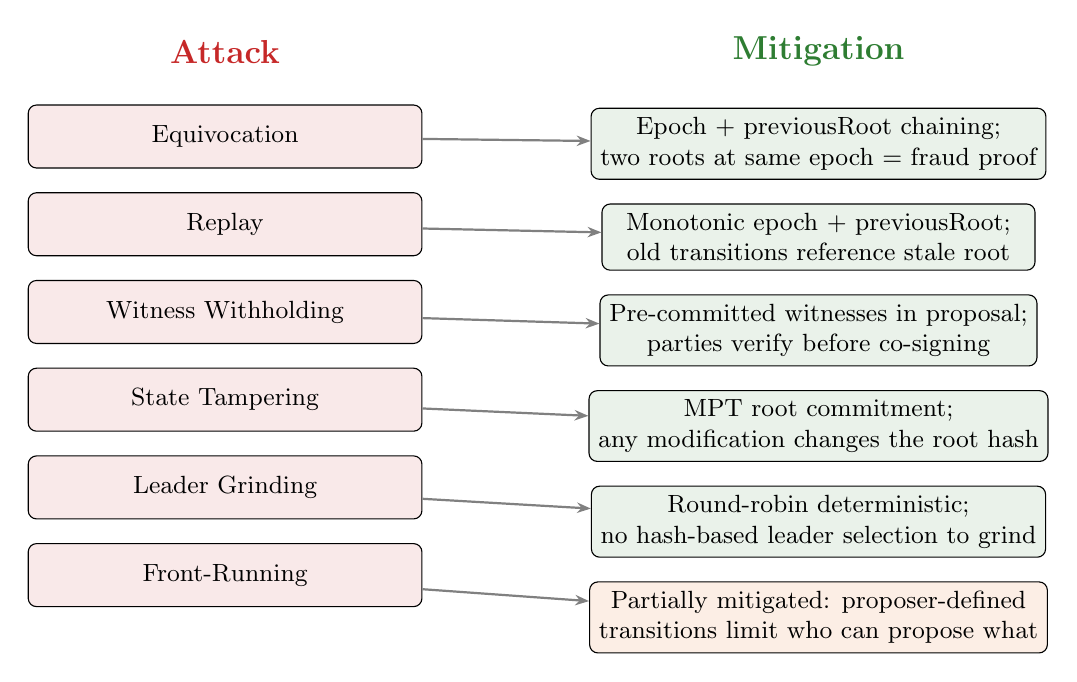
\begin{tikzpicture}[
  node distance=0.9cm,
  threat/.style={draw, rounded corners=3pt, minimum width=5cm, font=\small,
    align=center, minimum height=0.8cm},
  defense/.style={draw, rounded corners=3pt, minimum width=5.5cm, font=\small,
    align=center, minimum height=0.8cm},
  arrow/.style={-{Stealth[length=5pt]}, thick}
]

  \node[font=\large\bfseries, text=cnred] (tt) {Attack};
  \node[font=\large\bfseries, text=cngreen, right=5.5cm of tt] (td) {Mitigation};

  \node[threat, fill=cnred!10, below=0.4cm of tt] (t1) {Equivocation};
  \node[threat, fill=cnred!10, below=0.3cm of t1] (t2) {Replay};
  \node[threat, fill=cnred!10, below=0.3cm of t2] (t3) {Witness Withholding};
  \node[threat, fill=cnred!10, below=0.3cm of t3] (t4) {State Tampering};
  \node[threat, fill=cnred!10, below=0.3cm of t4] (t5) {Leader Grinding};
  \node[threat, fill=cnred!10, below=0.3cm of t5] (t6) {Front-Running};

  \node[defense, fill=cngreen!10, below=0.4cm of td] (d1)
    {Epoch + previousRoot chaining;\\two roots at same epoch = fraud proof};
  \node[defense, fill=cngreen!10, below=0.3cm of d1] (d2)
    {Monotonic epoch + previousRoot;\\old transitions reference stale root};
  \node[defense, fill=cngreen!10, below=0.3cm of d2] (d3)
    {Pre-committed witnesses in proposal;\\parties verify before co-signing};
  \node[defense, fill=cngreen!10, below=0.3cm of d3] (d4)
    {MPT root commitment;\\any modification changes the root hash};
  \node[defense, fill=cngreen!10, below=0.3cm of d4] (d5)
    {Round-robin deterministic;\\no hash-based leader selection to grind};
  \node[defense, fill=cnorange!10, below=0.3cm of d5] (d6)
    {Partially mitigated: proposer-defined\\transitions limit who can propose what};

  \draw[arrow, gray] (t1) -- (d1);
  \draw[arrow, gray] (t2) -- (d2);
  \draw[arrow, gray] (t3) -- (d3);
  \draw[arrow, gray] (t4) -- (d4);
  \draw[arrow, gray] (t5) -- (d5);
  \draw[arrow, gray] (t6) -- (d6);

\end{tikzpicture}
\caption{Threat model with mitigations. All critical attacks are addressed.
Front-running is partially mitigated via proposer restrictions.}
\label{fig:threats}
\end{figure}

\subsubsection{Equivocation Detection}

If a leader signs two different roots $R_k$ and $R_k'$ at the same epoch $k$
with the same \texttt{previousRoot}, both signatures constitute an
\textbf{equivocation proof}:

\[
  \text{EquivocationEvidence} = \big(
    \text{sig}_1(R_{k-1}, R_k, k),\;
    \text{sig}_2(R_{k-1}, R_k', k),\;
    R_k \neq R_k'
  \big)
\]

Any party holding both signatures can prove the leader acted maliciously.
In Phase~1, this triggers social ejection (parties refuse to continue the
protocol with the equivocator). In future phases, this could trigger
on-chain slashing.

\subsubsection{Witness Pre-Commitment}

The leader \emph{must} include MPT inclusion proofs for all state paths read
during transition validation as part of the proposal. This eliminates the
withholding attack entirely:

\begin{itemize}[nosep]
  \item Co-signers verify witnesses against $R_{k-1}$ before signing.
  \item If the leader omits a witness, co-signers reject the proposal.
  \item All co-signers hold the witnesses at signing time --- no party can
    later claim inability to produce evidence.
\end{itemize}

\subsubsection{ECDSA Signature Considerations}

The protocol uses independent ECDSA signatures (one per party) aggregated
in the \texttt{proofs} array. Two important considerations:

\begin{enumerate}[nosep]
  \item \textbf{Low-s normalization}: ECDSA signatures are malleable --- given
    $(r, s)$, the signature $(r, n-s)$ is also valid. The SDK enforces
    $s \leq n/2$ to ensure signature uniqueness, preventing double-counting
    in quorum validation.
  \item \textbf{Key registration}: The genesis ceremony requires each member
    to sign a challenge nonce, proving knowledge of their private key. This
    prevents rogue key attacks where a malicious party registers a crafted
    public key.
\end{enumerate}


% ============================================================================
\section{Dispute Resolution}
\label{sec:disputes}
% ============================================================================

\subsection{Phase 1: Client-Side Dispute Resolution}

In Phase~1, dispute resolution is implemented entirely in the SDK. The process
is ``social'' --- evidence is presented to all parties, and the honest
majority acts on it.

\begin{enumerate}[nosep]
  \item \textbf{Evidence Collection}: The disputing party compiles:
    \begin{itemize}[nosep]
      \item The last DED-committed root and epoch (Layer~2 anchor)
      \item The disputed proposal with all co-signatures
      \item The state witnesses from the proposal
      \item Their independent computation of the correct post-state root
    \end{itemize}

  \item \textbf{Verification}: Any party (or third-party auditor) can verify:
    \begin{itemize}[nosep]
      \item Download the diff bundle from DED storage
      \item Verify witnesses against the committed pre-state root
      \item Re-execute the transition function (from the code reference)
      \item Compare the computed post-state root with the disputed root
    \end{itemize}

  \item \textbf{Resolution}: The honest majority refuses to co-sign further
    transitions with the misbehaving party. The protocol forks: honest parties
    continue from the last valid state; the dishonest party is excluded.
\end{enumerate}

\begin{codebox}{typescript}
// Dispute evidence generation
const evidence = await protocol.generateDisputeEvidence({
  disputedEpoch: 42,
  myComputedRoot: 'abc123...',  // What I think the root should be
});
// evidence: { anchor, proposal, witnesses, myComputation, signatures }

// Dispute verification (can run on any party or auditor)
const verdict = await Protocol.verifyDispute(evidence, codeRef);
// verdict: { valid: true, correctRoot: 'abc123...', faultyParty: 'leader-pubkey' }
\end{codebox}

\subsection{Phase 2: Arbiter Service}

In Phase~2, an independent arbiter service can verify disputes without
requiring all parties to be online:

\begin{itemize}[nosep]
  \item The arbiter downloads committed state and diffs from DED.
  \item The arbiter loads and executes the transition function from the code
    reference.
  \item The arbiter publishes a signed verdict as a DED fingerprint, creating
    an on-chain record of the dispute outcome.
  \item Trust assumption: the arbiter is honest. Multiple independent arbiters
    can be used for redundancy.
\end{itemize}


% ============================================================================
\section{Sigma Protocols and Zero-Knowledge Proofs}
\label{sec:sigma}
% ============================================================================

\begin{researchbox}{Research Direction --- Not Included in Phases 1--2}
This section describes future cryptographic extensions that are
\textbf{not part of the initial implementation}. They are documented here
to establish the research direction and ensure the v1/v2 architecture does
not preclude their future addition.
\end{researchbox}

\subsection{The Vision}

In a multi-party protocol, parties may need to prove properties about their
local state without revealing the state itself. For example:

\begin{itemize}[nosep]
  \item ``My balance at \texttt{/state/alice/balance} is $\geq$ 100'' without
    revealing the exact balance.
  \item ``I hold a credential at \texttt{/state/alice/credentials/X}'' without
    revealing the credential details.
  \item ``The sum of all party balances under \texttt{/state/*/balance} equals
    the value at \texttt{/shared/total\_supply}'' (conservation invariant).
\end{itemize}

\subsection{Sigma Protocol Primer}

A sigma protocol ($\Sigma$-protocol) is a three-move interactive proof between
a Prover (P) and Verifier (V):

\begin{enumerate}[nosep]
  \item \textbf{Commitment}: P sends a random commitment $a$
  \item \textbf{Challenge}: V sends a random challenge $e$
  \item \textbf{Response}: P sends a response $z$ computed from $a$, $e$,
    and the secret witness
\end{enumerate}

\noindent The protocol satisfies \emph{completeness} (honest provers always
convince), \emph{special soundness} (extractable witness from two transcripts),
and \emph{honest-verifier zero-knowledge} (simulatable without the witness).

Via the \textbf{Fiat-Shamir transform}, interactive sigma protocols become
non-interactive by replacing the verifier's challenge with
$e = \text{H}(a \| \text{statement})$.

\subsection{Composition with MPT Proofs}

Sigma protocols compose naturally via AND and OR constructions:

\begin{itemize}[nosep]
  \item \textbf{AND}: Prove knowledge of witnesses $w_1$ AND $w_2$ by running
    both protocols in parallel with the same challenge.
  \item \textbf{OR}: Prove knowledge of $w_1$ OR $w_2$ (without revealing
    which) by simulating one protocol and running the other honestly.
\end{itemize}

\noindent For MPT state proofs, the compound statement would be:

\[
  \text{``I know } v \text{ at path } p \text{ in trie with root } R
  \text{, and } v \geq \text{threshold''}
\]

\subsection{Feasibility Assessment}

\begin{table}[H]
\centering
\begin{tabularx}{\textwidth}{lccX}
\toprule
\textbf{Approach} & \textbf{Proof Size} & \textbf{Verify Time} & \textbf{Feasibility} \\
\midrule
Pedersen + Bulletproofs & $\sim$700 B & $\sim$3 ms &
  Practical for range proofs on committed values. Requires storing Pedersen
  commitments alongside SHA-256 hashes in leaves. Does NOT prove MPT inclusion
  in ZK --- the inclusion proof is public. \\[8pt]
SNARK (SHA-256 circuit) & $\sim$200 B & $\sim$5 ms &
  Proves full MPT inclusion + property in ZK. But SHA-256 costs $\sim$25K R1CS
  constraints per hash; depth-8 MPT $\approx$ 200K constraints. Proof
  generation: seconds to minutes. \\[8pt]
SNARK (Poseidon hash) & $\sim$200 B & $\sim$5 ms &
  Poseidon costs $\sim$300 constraints per hash. Depth-8 MPT $\approx$ 2.4K
  constraints. Practical, but requires replacing the MPT hash function.
  \textbf{Breaking change.} \\[8pt]
WASM in ZK (zkWASM) & varies & varies &
  Prove correct execution of arbitrary WASM in ZK. Experimental; proof
  generation is very slow. Long-term research direction. \\
\bottomrule
\end{tabularx}
\caption{Zero-knowledge proof approaches and their feasibility for MPT state
proofs.}
\label{tab:zk}
\end{table}

\subsection{Recommended Path}

\begin{enumerate}[nosep]
  \item \textbf{Phase 3a}: Introduce Pedersen commitments as an optional leaf
    value type. Store $(\text{SHA-256}(v), \text{Pedersen}(v, r))$ in leaves.
    Enable Bulletproofs range proofs on committed values. The SHA-256 hash
    preserves backward compatibility; the Pedersen commitment enables ZK
    property proofs.
  \item \textbf{Phase 3b}: Evaluate algebraic hash migration (Poseidon) in
    the Tessellation MPT layer for full in-circuit verification. This is a
    multi-quarter effort affecting the entire Constellation stack.
  \item \textbf{Phase 3c}: Explore recursive SNARKs for compressing the entire
    protocol history into a single proof (``this root $R_k$ is the result of
    $k$ valid transitions from genesis'').
\end{enumerate}


% ============================================================================
\section{API Surface}
\label{sec:api}
% ============================================================================

\begin{codebox}{typescript}
import { WorldState } from '@constellation-network/ded-agent-worldstate';
import { Protocol } from '@constellation-network/ded-agent-worldstate/protocol';
import { supplyChainSpec } from '@acme/supply-chain-protocol';

// --- Initialize WorldState (same as v1) ---
const ws = await WorldState.create({
  privateKey: process.env.PRIVATE_KEY!,
  orgId: 'org-uuid',
  baseUrl: 'https://api.ded.example.com',
  apiKey: 'api-key',
  storagePath: './state',
});

// --- Create or join a protocol instance ---
const protocol = await ws.protocol(supplyChainSpec, {
  instanceId: 'handoff-2026-001',
  myRole: 'shipper',
  transport: myWebSocketTransport,  // User-provided
});

// --- Genesis (first party initiates) ---
await protocol.genesis({
  agreementHash: sha256(termsDocument),
});
// Waits for all members to co-sign genesis root

// --- Propose a transition ---
const proposal = await protocol.propose('shipment_dispatched', {
  trackingId: 'TRACK-12345',
  dispatchedAt: new Date().toISOString(),
  items: [{ sku: 'WIDGET-A', quantity: 100 }],
});
// Returns: { proposalId, epoch, previousRoot, newRoot, signatures }

// --- Listen for proposals (other party) ---
protocol.on('proposal', async (proposal) => {
  // SDK auto-validates: schema, witnesses, transition execution, root
  // If valid, proposal.autoValidated === true
  await protocol.sign(proposal.id);
});

// --- Read state ---
const value = await protocol.read('/state/shipper/dispatches/TRACK-12345');
const root = protocol.currentRoot();
const epoch = protocol.currentEpoch();

// --- Generate and verify proofs ---
const proof = await protocol.prove('/state/shipper/dispatches/TRACK-12345');
const valid = await Protocol.verifyProof(proof, protocol.currentRoot());

// --- Protocol lifecycle events ---
protocol.on('committed', ({ epoch, root, fingerprintHash }) => {
  console.log(`Epoch ${epoch} committed to DED: ${fingerprintHash}`);
});

protocol.on('finalized', ({ epoch, globalSnapshotOrdinal }) => {
  console.log(`Epoch ${epoch} finalized on-chain at snapshot ${globalSnapshotOrdinal}`);
});

protocol.on('dispute', ({ epoch, evidence }) => {
  console.log(`Dispute raised at epoch ${epoch}`);
});

// --- Dispute resolution ---
const evidence = await protocol.generateDisputeEvidence({ disputedEpoch: 5 });
const verdict = await Protocol.verifyDispute(evidence, supplyChainSpec.codeRef);

// --- Protocol state inspection ---
const info = await protocol.info();
// { epoch, root, members, lastCheckpointEpoch, lastCheckpointHash }
\end{codebox}


% ============================================================================
\section{Protocol Upgrades}
\label{sec:upgrades}
% ============================================================================

Protocol rules may need to change over time: adding members, modifying
transition schemas, or updating the code reference. Upgrades follow a
structured process:

\begin{enumerate}[nosep]
  \item A member proposes an upgrade by submitting a new \texttt{ProtocolSpec}
    with incremented \texttt{version}.
  \item The upgrade proposal is a special transition type
    (\texttt{protocol\_upgrade}) that \emph{always requires unanimity},
    regardless of the configured quorum.
  \item On unanimous approval:
    \begin{itemize}[nosep]
      \item The current protocol state is checkpointed to DED.
      \item The \texttt{/protocol/code} and \texttt{/protocol/config} paths
        are updated in the MPT.
      \item The new spec hash is recorded in \texttt{/audit/log/\{epoch\}}.
      \item Subsequent transitions use the new spec's rules.
    \end{itemize}
  \item The old spec hash remains in the audit trail, enabling verification
    of historical transitions against the rules that were active at the time.
\end{enumerate}

\begin{codebox}{typescript}
// Propose a protocol upgrade
const newSpec = {
  ...currentSpec,
  version: 2,
  members: {
    ...currentSpec.members,
    auditor: { publicKey: auditorPubKey, roles: ['read-only'] },
  },
};

await protocol.proposeUpgrade(newSpec);
// Requires all existing members to co-sign
\end{codebox}


% ============================================================================
\section{Implementation Roadmap}
% ============================================================================

\begin{table}[H]
\centering
\begin{tabularx}{\textwidth}{clX}
\toprule
\textbf{Phase} & \textbf{Deliverable} & \textbf{Description} \\
\midrule
0 & v1 WorldState & Single-party streams, chain linking, checkpoint/recovery,
  LevelDB persistence, DED integration. \emph{(Prerequisite, per v1
  proposal.)} \\[8pt]
1 & Bilateral Protocols & Two-party protocol instances. Transport interface.
  Genesis ceremony. Propose/sign lifecycle. State diff upload via
  \texttt{/upload}. Audit log. Client-side dispute evidence generation.
  Round-trip test suite with in-memory transport. \\[8pt]
2 & N-Party Protocols & Configurable quorum ($2f+1$). Round-robin leader
  election with timeout. N-party signature collection. State sync for late
  joiners (replay from DED). Protocol upgrades (member add/remove, code
  update). \\[8pt]
3a & Pedersen Commitments & Optional dual-commit leaves
  $(\text{SHA-256}, \text{Pedersen})$. Bulletproofs range proofs on committed
  values. Does not require server-side changes. \\[8pt]
3b & WASM Transitions & WebAssembly transition functions for cross-platform
  determinism. \texttt{codeRef} gains \texttt{type: ``wasm''} variant. \\[8pt]
3c & Algebraic Hash MPT & Poseidon-based MPT for SNARK-friendly inclusion
  proofs. Full compound ZK proofs: ``value at path $p$ in trie $R$ satisfies
  predicate $P$.'' \emph{Requires Tessellation-level changes.} \\
\bottomrule
\end{tabularx}
\caption{Implementation roadmap. Each phase builds on the previous.}
\label{tab:roadmap}
\end{table}


% ============================================================================
\section{Comparison with Related Systems}
% ============================================================================

\begin{table}[H]
\centering
\small
\begin{tabularx}{\textwidth}{lXXXX}
\toprule
& \textbf{MPVSP on DED} & \textbf{State Channels} & \textbf{Optimistic Rollups}
  & \textbf{zk-Rollups} \\
\midrule
\textbf{State} & Arbitrary MPT & Balance pairs & EVM state & EVM state \\
\textbf{Parties} & N (2--10) & 2 (bilateral) & Sequencer + verifiers
  & Sequencer + prover \\
\textbf{Off-chain speed} & Sub-second & Instant & N/A (all on-chain)
  & N/A \\
\textbf{Finality} & Minutes (DED batch) & Hours (dispute) & $\sim$7 days
  & Hours (proof gen) \\
\textbf{Dispute} & Client-side + arbiter & On-chain contract & Fraud proofs
  & Validity proofs \\
\textbf{DA} & DED S3 (diffs) & Parties only & L1 calldata & L1 calldata \\
\textbf{Trust} & Quorum of N & Both parties & 1-of-N honest & Cryptographic \\
\textbf{Cost/tx} & \$0.003 amortized & \$0 off-chain & \$0.01--0.10
  & \$0.01--0.10 \\
\textbf{Infra} & DED API only & L1 smart contract & L1 + L2 nodes
  & L1 + prover \\
\bottomrule
\end{tabularx}
\caption{Comparison with existing multi-party state systems.}
\label{tab:comparison}
\end{table}

\noindent \textbf{MPVSP's unique position}: It requires no smart contracts,
no L1 gas, no staking, and no specialized infrastructure beyond a DED API
key. The tradeoff is weaker dispute enforcement (social/arbiter-based rather
than on-chain automated). This makes MPVSP ideal for \emph{cooperative
multi-party workflows} (supply chain, compliance, escrow) where parties have
real-world relationships, rather than \emph{adversarial trustless} settings.


% ============================================================================
\section*{Appendix A: Cryptographic Commitment Properties}
% ============================================================================
\addcontentsline{toc}{section}{Appendix A: Cryptographic Commitment Properties}

The MPVSP inherits the DED MPT's cryptographic properties:

\begin{description}[leftmargin=2cm, style=nextline]
  \item[Binding]
    SHA-256 with type-prefix domain separation (0x00, 0x01, 0x02) ensures that
    two different sets of (path, value) pairs produce different root hashes
    with overwhelming probability ($2^{-256}$). The deterministic insertion
    order (confirmed by the \texttt{MptInsertionOrderDeterminismSuite} in the
    Tessellation test suite) guarantees that the root is uniquely determined by
    the logical content, not the insertion sequence.

  \item[Hiding]
    The MPT commits to \emph{hashes} of values, not plaintext. Leaf nodes
    store $\text{SHA-256}(v)$, not $v$ itself. However, the trie structure
    leaks metadata: Branch nodes reveal which path prefixes are populated, and
    Extension nodes reveal shared path segments. Future Pedersen commitment
    integration (Phase~3a) would add computational hiding for leaf values.

  \item[Non-Repudiation]
    Each party's signature is independently verifiable via SECP256K1. A party
    that co-signs a root cannot later deny having agreed to that state. The
    \texttt{SignedTransitionEnvelope} binds the signature to a specific
    (instance, epoch, previousRoot, newRoot) tuple, preventing signature
    reuse across different protocol contexts.

  \item[Temporal Ordering]
    The epoch counter provides a total order on transitions within a protocol
    instance. The previousRoot chaining ensures that the order is cryptographically
    enforced: skipping or reordering epochs would break the hash chain.
\end{description}


% ============================================================================
\section*{Appendix B: DED Fingerprint Encoding}
% ============================================================================
\addcontentsline{toc}{section}{Appendix B: DED Fingerprint Encoding}

Protocol state commitments are encoded in the existing DED \texttt{FingerprintValue}
fields without requiring schema changes:

\begin{table}[H]
\centering
\begin{tabularx}{\textwidth}{llX}
\toprule
\textbf{Field} & \textbf{MPVSP Usage} & \textbf{Notes} \\
\midrule
\texttt{orgId} & Organization UUID & Unchanged from v1 \\
\texttt{tenantId} & Protocol instance UUID & Derived from instanceId \\
\texttt{eventId} & Random UUID per checkpoint & Unique per fingerprint \\
\texttt{documentId} & \texttt{mpvsp:\{instanceId\}:epoch:\{N\}} & Protocol chain
  linking; epoch is monotonic \\
\texttt{documentRef} & Protocol MPT root hash (64 hex) & The agreed state root \\
\texttt{signerId} & Leader's public key & Proposing party \\
\texttt{timestamp} & ISO 8601 & Time of checkpoint submission \\
\texttt{version} & 1 & Schema version \\
\texttt{tags} & \texttt{protocol\_id}, \texttt{spec\_hash}, \texttt{epoch},
  \texttt{quorum} & Searchable metadata (max 6 tags) \\
\texttt{proofs} & All co-signer signatures & Quorum evidence \\
\bottomrule
\end{tabularx}
\caption{Mapping of MPVSP protocol data to DED fingerprint fields.}
\label{tab:encoding}
\end{table}


% ============================================================================
\section*{Appendix C: Open Questions}
% ============================================================================
\addcontentsline{toc}{section}{Appendix C: Open Questions}

\begin{enumerate}
  \item \textbf{Transition function determinism}: JavaScript has known
    non-determinism across runtimes (floating-point, string collation,
    Map iteration order). Should the SDK enforce a deterministic subset of
    JS, or mandate WASM from the start? \emph{Current decision: JS with RFC~8785
    canonical JSON for all state serialization; WASM as Phase~3b.}

  \item \textbf{Key rotation}: The genesis ceremony binds member identities
    to specific SECP256K1 keys. A \texttt{key\_rotation} transition type
    should allow a member to replace their key by co-signing with both old
    and new keys. This is not yet designed.

  \item \textbf{Partial state visibility}: In some protocols, parties should
    not see each other's private state paths. The current MPT structure leaks
    path existence via Branch nodes. Encrypted leaves or separate per-party
    tries with cross-references may be needed.

  \item \textbf{Cross-protocol references}: Can one protocol instance
    reference another's committed state? E.g., ``this escrow protocol's
    delivery confirmation references tracking proof from the logistics
    protocol.'' This would require cross-instance MPT proof verification.

  \item \textbf{FROST threshold signatures}: For Phase~3, migrating from
    independent ECDSA to FROST (Flexible Round-Optimized Schnorr Threshold)
    would produce constant-size signatures (64 bytes regardless of $N$) with
    native threshold semantics. This requires adding Schnorr support to the
    Constellation signing stack.

  \item \textbf{On-chain dispute enforcement}: Phase~1--2 rely on social
    enforcement. For high-value protocols, on-chain enforcement (metagraph
    validator extensions to check equivocation proofs and apply penalties)
    would provide stronger guarantees. This requires changes to the
    metagraph's \texttt{CalculatedState} and \texttt{Validator}.
\end{enumerate}


\end{document}
